\subsection{Onde o erro se concentra}
\label{sec:onde_erro}

O erro 3-D por evento cai com a luz detectada: a correlação de postos de Spearman $\rho_{\mathrm{S}}$ vale \num{-0.68} no GATv2-cascata e \num{-0.72} no XGBoost na luz limpa. Por quartil de luz do teste (limites: \num{201}, \num{387} e \qty{773}{\pe}), o erro 3-D médio do GATv2-cascata é de \num{42.79}, \num{31.25}, \num{18.19} e \qty{11.67}{\cm}, e o do XGBoost, de \num{47.28}, \num{35.74}, \num{20.78} e \qty{6.98}{\cm} (Figura~\ref{fig:erro_luz}): o GATv2-cascata erra menos nos três mais escuros (diferenças pareadas com intervalos acima de zero), e o XGBoost, \qty{4.70}{\cm} menos no mais claro (\num{3.58} a \qty{5.75}{\cm}). Os centroides com peso quadrático e linear respondem, respectivamente, por \num{43.5} e \qty{33.3}{\percent} da importância por ganho do XGBoost, treinado em luz com aumento. Como ambos ganham precisão com a luz, isso condiz com a vantagem nos eventos claros, mas não a explica: o GATv2\discretionary{-}{-}{-}cascata recebe os mesmos dois centroides entre os escalares do evento (Seção~\ref{sec:dados_grafos}), e a causa de seu erro maior nesses eventos não foi investigada.

No referencial dos sensores, o eixo $y$, normal às paredes longas, tem o menor RMSE no GATv2-cascata (\qty{14.35}{\cm}, contra \num{20.45} e \qty{20.46}{\cm} em $x$ e $z$), no GPS, nos \textit{boosters} na luz limpa e na rede da etapa anterior (eixos convertidos por correspondência inferida; Tabela~\ref{tab:referencias}). O eixo $x$, normal às faces sem canais, tem o maior nos \textit{boosters} (XGBoost: \qty{23.82}{\cm}) e naquela rede (\qty{24.68}{\cm}). O coeficiente de determinação $R^2$ do GATv2-cascata em $z$, fração da variância explicada, é \num{0.9994} porque o desvio-padrão dos vértices de teste é \num{4.6} vezes maior em $z$ que em $x$, não porque $z$ seja mais bem reconstruído.

Abaixo de $z = {}$\qty{20}{\m} (\num{626} eventos), os RMSE em $z$ do baricentro calibrado, do GATv2\discretionary{-}{-}{-}cascata e do XGBoost na luz limpa são próximos (\num{23.29}, \num{22.54} e \qty{22.63}{\cm}); a partir de \qty{20}{\m} (\num{311} eventos), o do baricentro sobe para \qty{65.87}{\cm}, e os outros dois caem para \num{15.44} e \qty{18.91}{\cm} (Figura~\ref{fig:erro_z}). O fator \num{2.07} da Seção~\ref{sec:comparacao_referencias} vem desses vértices: os canais da tampa, todos em $z = {}$\qty{29.93}{\m}, recebem \qty{41.2}{\percent} da luz e deslocam o baricentro tanto mais quanto mais longe o vértice está das paredes longas, o que a calibração, função só de $\bar{z}$, não corrige.

\begin{figure}[H]
  \centering
  \begin{subfigure}[t]{0.485\textwidth}
    \centering
    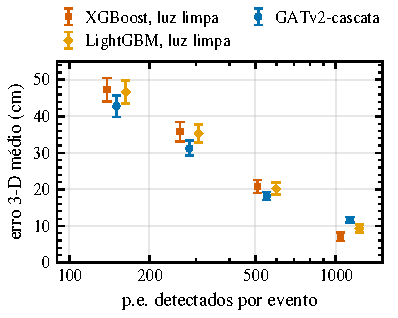
\includegraphics{figures/erro_luz.pdf}
    \caption{Erro 3-D médio do GATv2\discretionary{-}{-}{-}cascata e, na luz limpa, do \mbox{XGBoost} e do \mbox{LightGBM}, por quartil da luz detectada nos \num{937} eventos de teste; pontos na luz média do quartil, os dos \textit{boosters} deslocados para os lados, e barras de \qty{95}{\percent} de cada média, por \textit{boot\-strap} sobre os eventos do quartil. O GATv2\discretionary{-}{-}{-}cascata erra menos nos três mais escuros, e o \mbox{XGBoost}, no mais claro (\qty{773}{\pe} ou mais); o intervalo da diferença pareada entre os dois exclui o zero em todos os quartis.}
    \label{fig:erro_luz}
  \end{subfigure}\hfill
  \begin{subfigure}[t]{0.485\textwidth}
    \centering
    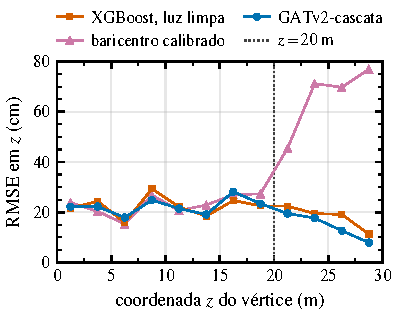
\includegraphics{figures/erro_z.pdf}
    \caption{RMSE em $z$ do GATv2-cascata, do baricentro calibrado e do \mbox{XGBoost} na luz limpa nos eventos de teste, por faixa de \qty{2.5}{\m} do $z$ do vértice; linha pontilhada em \qty{20}{\m}. Até \qty{20}{\m}, os erros são próximos; perto da tampa ($z = {}$\qty{29.93}{\m}), o do baricentro sobe e o do GATv2-cascata cai.}
    \label{fig:erro_z}
  \end{subfigure}
  \caption{Onde o erro se concentra nos eventos de teste: (a)~por quartil de luz detectada; (b)~por faixa de $z$ do vértice.}
  \label{fig:par_onde_erro}
\end{figure}
